\chapter{Architecture logiciel}

\section{Architecture globale}

Le projet consiste à construire une bibliothèque permettant de générer plusieurs
types de cartes d'élévations (planes, sphériques) à l'aide de diverses
méthodes (fractales, bruits), et d'exporter ces dernières pour les visualiser sous des logiciels 
comme Terragen et Blender3D.

La figure \ref{fig:class-diagram} présente l'architecture que nous avons imaginé,
elle sera décrite plus en détails dans le chapitre suivant.

\begin{sidewaysfigure}
  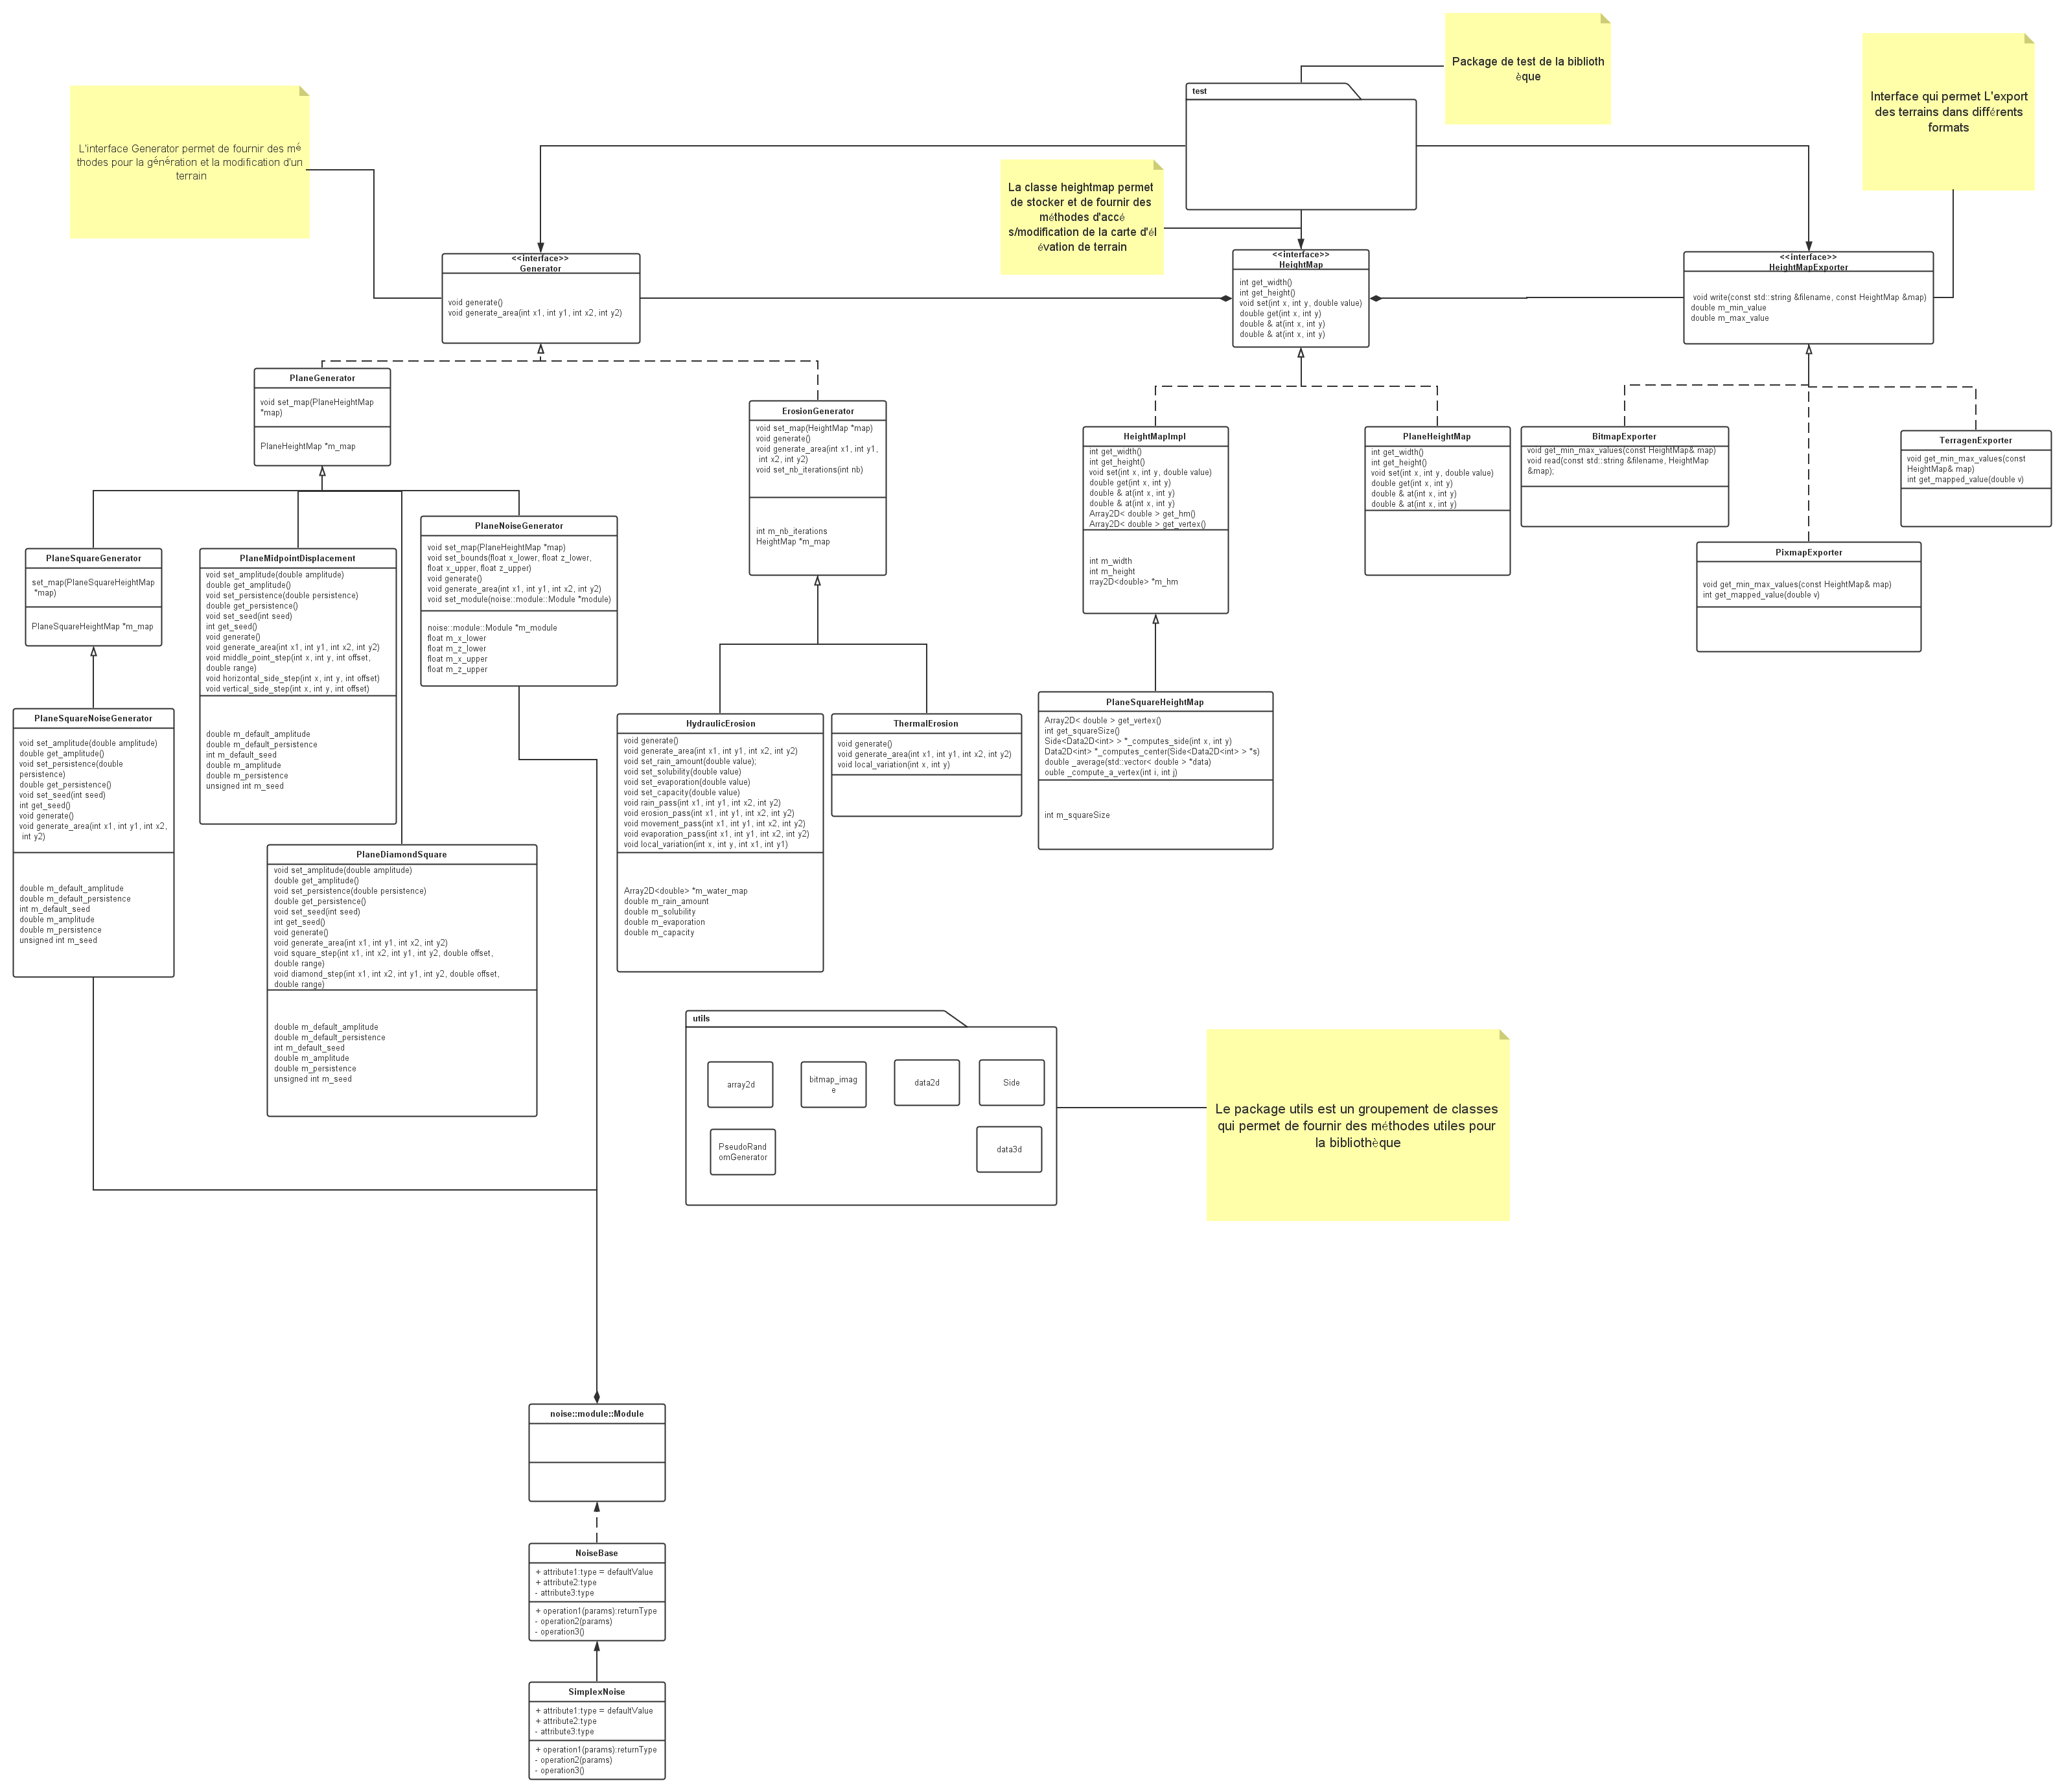
\includegraphics[width=20cm]{resources/Diag_Planetgen_v5.png}
        \caption{Diagramme de classe}
        \label{fig:class-diagram}
\end{sidewaysfigure}

On distingue ainsi 5 modules principaux :
\begin{itemize}
 \item la topologie de la carte d'élévation (classe heightMap);
 \item la génération des hauteurs de la carte;
 \item l'export de la carte;
 \item les classes utilitaires;
 \item les tests.
\end{itemize}

\section{Architecture des composants}

\subsection{Classe HeightMap}
Plusieurs classes implémentent cette interface. Intéressons nous aux deux premières classes : HeightMapImpl et PlanHeightMap.
La première est celle qui prendra en compte la topologie du terrain avec le type de grille choisi.
La seconde classe, elle, est utile pour itérer des algorithmes sans se soucier de la topologie et de la grille.
Il s'agit donc d'une classe servant à abstraire certaines informations dans le but de se concentrer sur 
l'implémentation des méthodes de génération. Cette classe est utilisée pour les tests.

\subsection{Classe Generator}
Deux classes implémentent cette interface. Il s'agit de PlaneGenerator et ErosionGenerator.
Avec différentes topologies, il pourrait exister des CubeGenerator, etc. Le PlaneGenerator permet
de factoriser le code nécessaire à la génération des cartes planaires. Les méthodes de bruits et les fractales
disposent d'implémentations différentes en s'adaptant au type de terrain. Concrètement, avec une carte sphérique, il faudrait 
prendre en compte l'influence des bordures de la carte sur les bordures opposées.
ErosionGenerator est à part car il prend en entré une carte d'élévation et donc il effectue des 
variations de hauteurs sur une topologie déjà existante.

\subsection{Classe HeightMapExporter}
Cette interface se contente de proposer à l'utilisateur plusieurs types d'exportation. 
L'export sous Blender3D n'a pas été rajouté car les résultats n'ont pas encore été étudiés suffisamment sur ce logiciel.

\subsection{Classes de tests (figure \ref{fig:class-diagram-test})}
Des classes de test ont été développées pour vérifier la génération des bruits.

\begin{sidewaysfigure}
  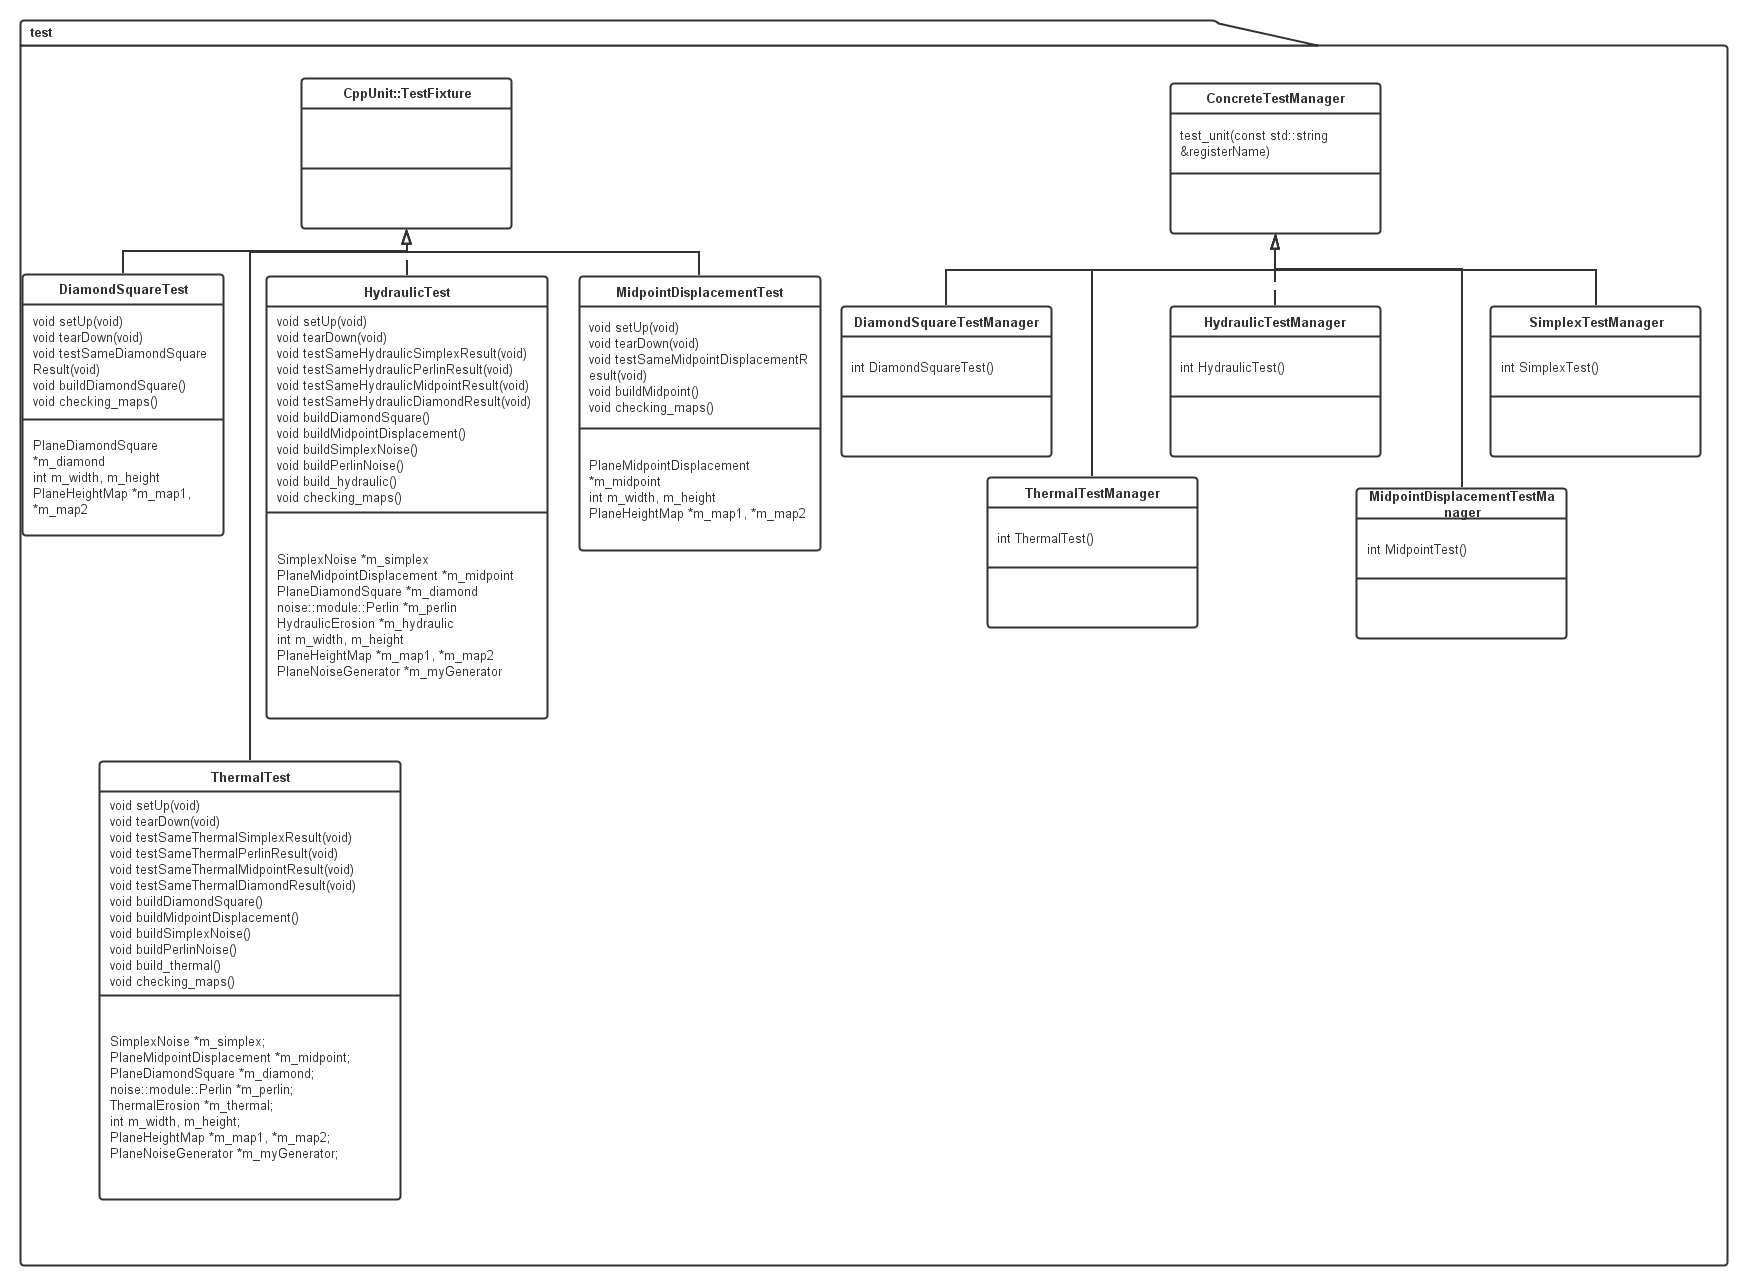
\includegraphics[width=20cm]{resources/Test_package_v2.png}
        \caption{Digramme de classe des Tests}
        \label{fig:class-diagram-test}
\end{sidewaysfigure}

Chaque méthode testée possède ses propres classes :
\begin{itemize}
 \item un manager. Il sert à remplir le registre de cppunit dédié à la méthode de génération en cours de test.
 Dans ce registre dédié, il est possible de rajouter plusieurs classes de tests pour une même méthode de génération 
  (exemple : DiamondPerf, DiamondPersistance, etc);
 \item les classes de test. Chaque classe enchaîne les tests \textit{via} les macros de cppunit.
\end{itemize}

\subsection{Classes utilitaires}
Ces classes sont des structures de données implémentées dans l'objectif de simplifier le code des 
sources.



